\let\negmedspace\undefined
\let\negthickspace\undefined
\documentclass[journal]{IEEEtran}
\usepackage[a5paper, margin=10mm, onecolumn]{geometry}
%\usepackage{lmodern} % Ensure lmodern is loaded for pdflatex
\usepackage{tfrupee} % Include tfrupee package

\setlength{\headheight}{1cm} % Set the height of the header box
\setlength{\headsep}{0mm}     % Set the distance between the header box and the top of the text

\usepackage{gvv-book}
\usepackage{gvv}
\usepackage{cite}
\usepackage{amsmath,amssymb,amsfonts,amsthm}
\usepackage{algorithmic}
\usepackage{graphicx}
\usepackage{textcomp}
\usepackage{xcolor}
\usepackage{txfonts}
\usepackage{listings}
\usepackage{enumitem}
\usepackage{mathtools}
\usepackage{gensymb}
\usepackage{comment}
\usepackage[breaklinks=true]{hyperref}
\usepackage{tkz-euclide} 
\usepackage{listings}
% \usepackage{gvv}                                        
\def\inputGnumericTable{}                                 
\usepackage[latin1]{inputenc}                                
\usepackage{color}                                            
\usepackage{array}                                            
\usepackage{longtable}                                       
\usepackage{calc}                                             
\usepackage{multirow}                                         
\usepackage{hhline}                                           
\usepackage{ifthen}                                           
\usepackage{lscape}
\usepackage{multicol}
\begin{document}

\bibliographystyle{IEEEtran}
\vspace{3cm}

\title{3.0.12}
\author{EE25BTECH11012-BEERAM MADHURI}
% \maketitle
% \newpage
% \bigskip
{\let\newpage\relax\maketitle}

\renewcommand{\thefigure}{\theenumi}
\renewcommand{\thetable}{\theenumi}
\setlength{\intextsep}{10pt} % Space between text and floats


\numberwithin{equation}{enumi}
\numberwithin{figure}{enumi}
\renewcommand{\thetable}{\theenumi}


\textbf{Question}:\\
A loaded dice has following probability distribution of occurrences

\begin{center}
\begin{tabular}{|c|c|c|c|c|c|c|}
\hline
Dice value & 1 & 2 & 3 & 4 & 5 & 6 \\
\hline
Probability & $\frac{1}{4}$ & $\frac{1}{8}$ & $\frac{1}{8}$ & $\frac{1}{8}$ & $\frac{1}{8}$ & $\frac{1}{4}$ \\
\hline
\end{tabular}
\end{center}

If three identical dice as the above are thrown, the probability of occurrence of values $1, 5$ and $6$ on the three dice is \hfill (EE 2007)

\begin{enumerate}
\item[(a)] same as that of occurrence of $3, 4, 5$
\item[(b)] same as that of occurrence of $1, 2, 5$
\item[(c)] $\frac{1}{128}$
\item[(d)] $\frac{5}{8}$
\end{enumerate}

\textbf{Solution:}\\
The Probability of occurance of 1, 5, 6:\\
let,\\
A = Event that 1 appeared when the die with the given probability distribution is thrown.\\
B = Event that 5 appeared when the die with the given probability distribution is thrown.\\
C = Event that 6 appeared when the die with the given probability distribution is thrown.\\
\begin{align}
    P(A) = 1/4\\
    P(B) = 1/8\\
    P(C) =1/4
\end{align}
Occurence of 1-6 on each of the dice is independent of the output of the other.\\
$\therefore$A, B, C are independent of each of other.
\begin{align}
    P(A \cap B \cap C)=P(A) P(B)P(C)\\
    =(1/4)(1/8)(1/8)\\
    =1/128
\end{align}
$\therefore$ The Probability of occurance of 1, 5, 6=1/128

\textbf{Option A:}\\
Occurance of 3,4,5:\\
A = Event that 3 appeared when the die with the given probability distribution is thrown.\\
B = Event that 4 appeared when the die with the given probability distribution is thrown.\\
C = Event that 5 appeared when the die with the given probability distribution is thrown.\\
\begin{align}
    P(A \cap B \cap C)=P(A) P(B)P(C)\\
    =(1/8)(1/8)(1/8)\\
    =1/512
\end{align}

\textbf{Option B:}\\
Occurance of 1,2,5:\\
A = Event that 1 appeared when the die with the given probability distribution is thrown.\\
B = Event that 2 appeared when the die with the given probability distribution is thrown.\\
C = Event that 5 appeared when the die with the given probability distribution is thrown.\\
\begin{align}
    P(A \cap B \cap C)=P(A) P(B)P(C)\\
    =(1/4)(1/8)(1/8)\\
    =1/256
\end{align}

Option (C) is correct.

\begin{figure}[H]
\centering
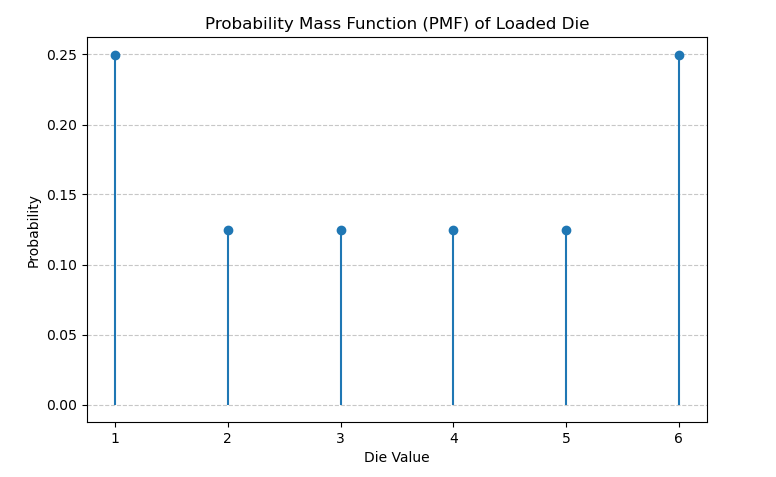
\includegraphics[width=0.75\columnwidth]{Figures/pmf.png}
\caption{PMF}
\label{fig:placeholder}
\end{figure}

The desired Probability is computed numerically by generating the distribution by rolling the dice 1000000 times.
\begin{figure}[H]
\centering
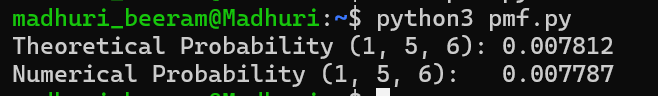
\includegraphics[width=0.75\columnwidth]{Figures/Numerical.png}
\caption{Output}
\label{fig:placeholder}
\end{figure}
Numerically found value closely matches with the calculated Probability.

\end{document}
